\section{Reduced Order Modeling}
\label{sec:ROMs}
To provide a very simple idea of a ROM, assume that the final
response space of a physical system is governed by the transfer
function $H \left (  \overline{x}\right)$ (see Section
~\ref{sec:mathBackground}), which, from a practical point of
view, represents the outcome of the system based on the initial
conditions  $\overline{x}$. Now, sample the domain of variability of the
initial conditions $\overline{x}$ to create a
set of $N$ realizations of the input and response space $ \left ( \left (
\overline{x}_{i}, H \left (  \overline{x}_{i}\right) \right), i=1,N \right)$,
named ``training'' set. Based on the data set generated, it is possible
to construct a mathematical representation $G\left ( \overline{x}:
\overline{x}_{i}\right)$ of the
real system $H \left (  \overline{x}\right)$, which will approximate its
response (see Figure~\ref{fig:ROMexampleOfPhysicalSystem}):
\begin{equation}
\label{eq:regressor}
G\left ( \overline{x} \right ):\overline{x}_{i} \rightarrow G\left ( \overline{x}_{i} \right ) \cong H\left ( \overline{x}_{i} \right )
\end{equation}
The ROMs reported above are generally named ``regressors'', among
which all the most common data fitting algorithms are found (e.g.,
least square for construction of linear models).
An important class of ROMs for the work presented here after is the
one containing the so called ``classifiers''. A classifier is a ROM that is
capable of representing the system behavior from a binary point of
view (e.g., event happened/not happened or failure/success). It is a
model (set of equations) that identifies to which category an object
belongs in the feature (input) space. Referring to the example that
brought to Equation ~\ref{eq:regressor}, a classifier can be formally represented as follows (see
Figure~\ref{fig:ROMClassifierExampleOfPhysicalSystem}):
\begin{figure}[h!]
  \centering
  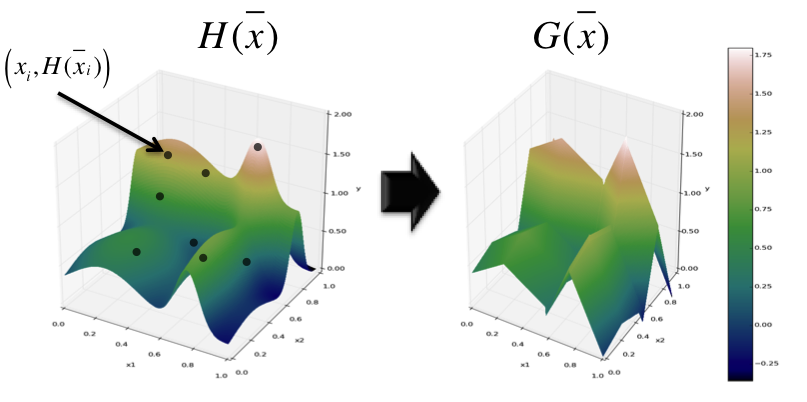
\includegraphics[width=1.0\textwidth]  {pics/ROMexampleOfPhysicalSystem.png}
  \caption{Example of reduced order model representation of physical system (regression).}
  \label{fig:ROMexampleOfPhysicalSystem}
\end{figure}
\begin{figure}[h!]
  \centering
  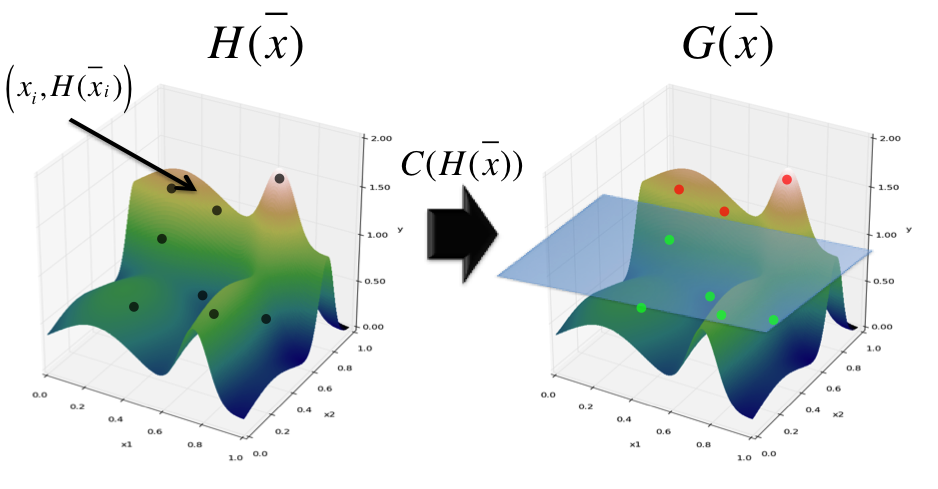
\includegraphics[width=1.0\textwidth]  {pics/ROMClassifierExampleOfPhysicalSystem.png}
  \caption{Example of reduced order model representation of physical system (classifier).}
  \label{fig:ROMClassifierExampleOfPhysicalSystem}
\end{figure}

\begin{equation}
\label{eq:classifier}
G\left ( \overline{x} \right ):\overline{x}_{i} \rightarrow G\left ( \overline{x}_{i} \right ) \cong
C \left ( H\left ( \overline{x}_{i} \right ) \right )
\end{equation}

The function $C\left (  H\left ( \overline{x}_{i}  \right ) = \overline{\theta}
\right ) $ is the so called ``goal'' function that is able to recast the
response of the system $H\left ( \overline{x}_{i}  \right )$ into a binary
form (e.g., failure/success). As an example, referring to
Figure~\ref{fig:ROMClassifierExampleOfPhysicalSystem}, the
``goal'' function would be:
\begin{equation}
\label{eq:goalFunctionClassifier}
C\left (   \overline{\theta}  \right ) = \left\{\begin{matrix}
1 & if \: \overline{\theta}>1.0 \\
0 &  if \: \overline{\theta} \leq 1.0
\end{matrix}\right.
\end{equation}
Hence, the ROM of type classifier $G\left (  \overline{x} \right )$  will operate in the space transformed through the ``goal''  function $C\left (   \overline{\theta}  \right )$.
\\The classifiers and regressors can be categorized into two main classes:
\begin{itemize}
  \item Model-based algorithms
  \item Data-based algorithms
\end{itemize}
In the first class, the created ROM aims to approximate the response
of the system as a function of the input parameters. These algorithms
construct a functional representation of the system. Examples of such ROM type are Support Vector Machines (SVMs), Kriging-based regressors, discriminant-based models, and polynomial chaos.

On the other side, data-based algorithms do not build a response-
function-based ROM but classify or predict the response of the
system from the neighborhood graph constructed from the training
data, without any dependencies on a particular prediction model.
These algorithms directly build a neighborhood structure as the
ROM (e.g., a relaxed Gabriel graph) on the initial training data. Examples of such ROM type are nearest neighbors and decision trees.

\textcolor{red}{\\It is important to NOTE that RAVEN uses a Z-score normalization of the training data before
  constructing most of the ROMs:
\begin{equation}
  \mathit{\mathbf{X}} = \frac{(\mathit{\mathbf{X}}-\mu )}{\sigma }
\end{equation}
 }
In order to identify which ROMs get trained with data normalized by the previous reported normalization approach, please refer to the RAVEN user manual \cite{RAVENuserManual}.

RAVEN has support of several different ROMs,
such as:
\begin{enumerate}
  \item \textit{Nearest Neighbors approaches}
  \item \textit{Support Vector Machines}
  \item \textit{Inverse Weight regressors}
  \item \textit{Spline regressors }, etc.
\end{enumerate}
In this section only few of them are going to be explained. 

\subsection{Gaussian Process Models}
\label{sec:GPM}
Gaussian Processes (GPs)~\cite{Rasmussen_GPM} are algorithms that extend multivariate Gaussian distributions to infinite dimensionality. A Gaussian process generates a data set located throughout some domain such that any finite subset of the range follows a multivariate Gaussian distribution. Now, the n observations in an arbitrary data set, $y={y_1,\ldots,y_n}$, can always be imagined as a single point sampled from some multivariate ($n$-variate) Gaussian distribution.
What relates one observation to another in such cases is just the covariance function, $k(x,x')$. A popular choice is the squared exponential:
\begin{equation}
k(x,x')=\sigma_{f}^{2}  exp \left [ \frac{-(x-x')^2}{2 l^2} \right ]
\end{equation}
where the maximum allowable covariance is defined as $\sigma_{f}^{2}$; this should be high for functions that cover a broad range on the y axis. If $x \simeq x'$, then $k(x,x')$ approach this maximum meaning $f(x)$ is very correlated to $f(x')$. On the other hand, if $x$ is very distant from $x'$, then $k(x,x' ) \simeq 0$ (i.e., the two points cannot see each other.
So, for example, during interpolation at new $x$ values, distant observations will have negligible effect). How much effect this separation has will depend on the length parameter $l$.
Each observation $y$ can be thought of as related to an underlying function $f(x)$ through a Gaussian noise model:
\begin{equation}
y=f(x)+N(0,\sigma_{n}^{2})
\end{equation}
The new kernel function can be written as:
\begin{equation}
k(x,x')=\sigma_{f}^{2}  exp \left [ \frac{-(x-x')^2}{2 l^2} \right ] + \sigma_{n}^{2} \delta(x,x')
\end{equation}
So given $n$ observations $y$, the objective is to predict the value $y_*$ at the new point $x_*$. This process is performed by following this sequence of steps:
\begin{enumerate}
\item Calculate three matrices:
\begin{equation}
K=\begin{bmatrix}
k(x_1,x_1) &  \ldots & k(x_1,x_n)\\
\vdots  & \ddots &\vdots  \\
k(x_n,x_1) &  \ldots & k(x_n,x_n)
\end{bmatrix}
\end{equation}
\begin{equation}
K_*= \begin{bmatrix}
k(x_*,x_1) & \ldots & k(x_*,x_n)
\end{bmatrix}
\end{equation}
\begin{equation}
K_{**}=k(x_*,x_*)
\end{equation}
\item The basic assumption of GPM is that:
\begin{equation}
\begin{bmatrix}
y\\
y_*
\end{bmatrix}
=\mathcal{N}(0,\begin{bmatrix}
K & K_{*}^{T}\\
K_* & K_{**}
\end{bmatrix})
\end{equation}
\item The estimate $\bar{y_*} $ for $y_*$ is the mean of this distribution
\begin{equation}
\bar{y_*}=K_* K^{-1}y
\end{equation}
\item The uncertainty associated to the estimate $\bar{y_*} $ can be expressed in terms of variance of  $y_*$:
\begin{equation}
var(y_*)=K_{**}-k_* K^{-1} K_{*}^{T}
\end{equation}
\end{enumerate}

\subsection{Support Vector Machines}
\label{sec:SVM}
The Support Vector Machine (SVM)~\cite{SVM_Burges} classifier is a methodology that aims to determine the optimal separation hyperplane between data sets having different labels.
The training data consist of $N$ data points $(x_i,y_i)$ $i=1,\ldots,N$ where $x_i \in \mathbb{R}^M$ and $y_i \in {-1,1}$.
Assuming a linear property of the hyperplane  then its definition is:
\begin{equation}
\left \{ x: f(x)=x^T\beta+\beta_0=0 \right \}
\end{equation}
where $\beta$ is a unit vector.

The SVM parameters $\beta$ and $\beta_0$  are determined by solving this optimization problem:
\begin{equation}
\left\{\begin{matrix}
\underset{\beta,\beta_0}{min} \left \| \beta \right \|\\
\text{subject to } y_i(x_{i}^{T}\beta+\beta_0)\geq 1 , \quad i=1,\dots,N
\end{matrix}\right.
\end{equation}

Once the SVM parameters $\beta$ and $\beta_0$ are determined then the classification of a new point $\bar{x}$ is given by:
\begin{equation}
G(\bar{x})=sign(\bar{x}^T\beta+\beta_0)
\end{equation}


\subsection{KNN Classifier and KNR Regressor}
\label{sec:KNN_KNR}
The K Nearest Neighbor algorithm~\cite{altman_KNN} (KNN) is a non-parametric method used for both regression and classification. The only input parameter is the variable $K$ which indicates the number of neighbors to be considered in the classification/regression process. The special case where the class is predicted to be the class of the closest training sample (i.e. when $K = 1$) is called the nearest neighbor algorithm. In binary (two class) classification problems, it is helpful to choose k to be an odd number as this avoids tied votes. The output depends on whether KNN is used for classification or regression:
\begin{itemize}
\item In KNN classification, the output is a class membership. An object is classified by a majority vote of its neighbors, with the object being assigned to the class most common among its $K$ nearest neighbors ($K$ is a positive integer, typically small). If $K = 1$, then the object is simply assigned to the class of that single nearest neighbor.
\item In KNN regression, the output is the property value for the object. This value is the average of the values of its $K$ nearest neighbors.
\end{itemize}
Both for classification and regression, it can be useful to assign weight to the contributions of the neighbors, so that the nearer neighbors contribute more to the average than the more distant ones. For example, a common weighting scheme consists in giving each neighbor a weight of $1/d$, where $d$ is the distance to the neighbor.

\subsection{Multi-Dimensional Interpolation}
\label{sec:ND_interp}
This section covers the methods that have been implemented in the CROW statistical library:
\begin{itemize}
\item Shepard's Method (see Section~\ref{sec:shepard})
\item Multi-Dimensional Spline method (see Section~\ref{sec:ND_spline}).
\end{itemize}

These two methods are interpolation methods that can be used in any dimension.
In RAVEN they are employed in two major applications:
\begin{enumerate}
\item ROMs
\item Multi-dimensional distributions.
\end{enumerate}
For both applications, given a set of $N$ data points $ (x_i,u_i )$  $i=1,\ldots,N$ where $x_i$ are the coordinate in the input space $D \subset \mathbb{R}^M$ and $u_i \in \mathbb{R}$ is the outcome, the methods predicts the outcome $\tilde{u}$ for a new coordinate $\tilde{x}\in \mathbb{R}^n$.


\subsubsection{Shepard's Method}
\label{sec:shepard}
The Shepard interpolator~\cite{Shepard} is also know as Inverse Distance Weighting (IDW) interpolator.
The starting point is a set of $N$ data points $ (x_i,u_i )$ for $i=1,\ldots,N$.
The Inverse-Weight interpolator can be represented as a function $f_{IDW}(x)$ that, given a new coordinate in the input space $x$, generates a prediction on $u$ such that
\begin{equation}
u:x \in \mathbb{R}^M \rightarrow f_{IDW}(x) \in \mathbb{R}
\end{equation}
based on the distance $d(x,x_i)$ in the euclidean space between $x$ and $x_i$.

Such prediction $u=f_{IDW}(x)$ is performed by summing all data points $x_i$ $i=1,\ldots,N$ weighted by a weighting parameter $w_i (x)$ as follows:
\begin{equation}
f_{IDW}(x) =
\left\{
\begin{matrix}
\sum_{i=1}^{N} w(x_i) u_i &  \text{if } d(x,x_i) \neq 0 \\
 u_i &  \text{if } d(x,x_i) = 0
\end{matrix}\right.
\end{equation}
where
\begin{equation}
w(x_i) =\frac{w_i}{\sum_{i=1}^{N} w_i}
\end{equation}
and
\begin{equation}
w_i = \left ( \frac{1}{d(x,x_i)} \right )^p
\end{equation}
Large values of $p$ assign greater weight $w_i$ to data points $x_i$ closest to $x$, with the result turning into a mosaic of tiles (i.e., Voronoi diagram) with nearly constant interpolated value.

\subsubsection{Multi-Dimensional Spline}
\label{sec:ND_spline}
The Multi-Dimensional Spline (MDS)~\cite{MD_spline} is a method that requires the sampled points $x_i$ to be lying in multi-dimensional cartesian grid.
A generic grid $\Delta_m$ for each dimension $m$ will be indicated as follows:
\begin{equation}
\Delta_m = \{x_{0_m},x_{1_m},\ldots,x_{p_m}\} \text{ for } m=1,\ldots,M
\end{equation}
This methods construct a $M$-dimensional cubic spline so that, given a coordinate in the input space $x=(x_1,x_2,\ldots,x_M)$, generates a prediction on $u$ such that
\begin{equation}
u:x \in \mathbb{R}^M \rightarrow f_{MDS}(x) \in \mathbb{R}
\end{equation}
where
\begin{equation}
f_{MDS}(x)=\sum_{i_1=1}^{p_1+3} \sum_{i_2=1}^{p_2+3} \ldots \sum_{i_M=1}^{p_M+3} c_{i_1,i_2,\ldots,i_p} \prod_{m=1}^{M} u_{i_j} (x_m)
\end{equation}
where
\begin{equation}
u_{i_j} (x_m) = \Phi\left ( \frac{x_m-x_{0_m}}{h_j}+2-i_j  \right )
\end{equation}

The cubic kernel $\Phi(t)$ is defined as:
\begin{equation}
\Phi(t) = \left\{\begin{matrix}
(2-\left | t \right |)^3 & 1\leq \left | t \right |\leq 2 \\
4-6\left | t \right |^2+3\left | t \right |^3 & \left | t \right |\leq 1\\
0 & \text{elsewhere}
\end{matrix}\right.
\end{equation}

The set of $\prod_{m=1}^{M}(p_m+3)$ coefficients $c_{i_1,i_2,\ldots,i_p}$  is determined when the interpolator is initialized.

